\chapter{应用语义关系自动构建情感词典}
\label{ch2}
%本章将进入论文排版的正文, 按元素分主要包括:
%{\kai 字体段落,图片表格,公式定理,参考文献}这几部分。
%这个样例文件将包括模板中使用到的所有格式、模板中自定义命令到或者特有的东西,
%都将被一一介绍,希望大家在排版自己的学位论文前能细致的看一遍,记住样例的格式和
%方法,方便上手。

\section{引言}
\label{ch2:intro}
上一章主要介绍了本文的研究背景,要研究的科学问题,研究内容与方法,并指出观点分析研究一项基础的工作就是研究如何针对不同应用构建具有足够覆盖面并且良好适应性的情感知识词典。人在使用语言表达情感或观点时,最基本的方式是使用具有明确情感色彩的词汇,因此为了分析用户的观点,最直接的方法应该从用户产生文本中使用的词语开始,将语言中经常使用的词语所表达的情感信息进行汇总形成的词典就是情感词典。观点分析研究首先是在英文文本上开始的,情感词典相关研究也是从英文为主,方法相对比较成熟,形成了一些经常使用的英文情感词典资源。中文情感分析研究起步较晚,缺乏普遍认可的可靠的中文情感词典\upcite{朱嫣岚2006,朱征宇2013,黄硕2013}。目前研究使用主要有HowNet情感词典\upcite{2013},NTUSD情感词典\upcite{Ku2007}以及大连理工大学的情感词汇本体词库\upcite{2013a}。这些词典主要是以手工或半自动方式编辑而成,覆盖度、可靠性和领域适应性受到限制,并且情感词以主要积极和消极二值区分,缺少情感极性值的细粒度划分。能够将资源丰富的英文词典中的情感知识跨语言向中文词典进行适应性的转化,构建相应的中文情感词典资源,既可以省去耗费大量人力的人工标注过程,又可以克服目前中文情感词典自动或半自动构建方法的可靠性和覆盖度问题。
因此本章提出将英文情感词典资源情感知识转化为中文情感词典的构建方法,可以根据语义关系将英文词语及其情感极性值转化得到中文词语的情感极性值,并且完全是自动的,可靠性更高。下一章将该方法构建的情感词典在领域语料中进行扩展,以提高其领域覆盖度和适应性。

本章具体安排如下:首先对情感词典构建需要考虑的问题以及相关工作进行全面的介绍,接着对本章要使用的词典资源进行介绍,然后详细阐述如何利用一个双语语义知识库将英文情感词典情感知识转化为中文情感词典相应的词语情感信息,最后对该方法进行实验验证和说明。

\section{相关工作}
构建情感词典需要考虑词典覆盖面(Coverage)、词典内容(Content)以及构建方法(Acquisition)三个方面问题,具体内容可以用图~\ref{fig2-1-1}框架来展示。

\begin{figure}[htp]
\centering
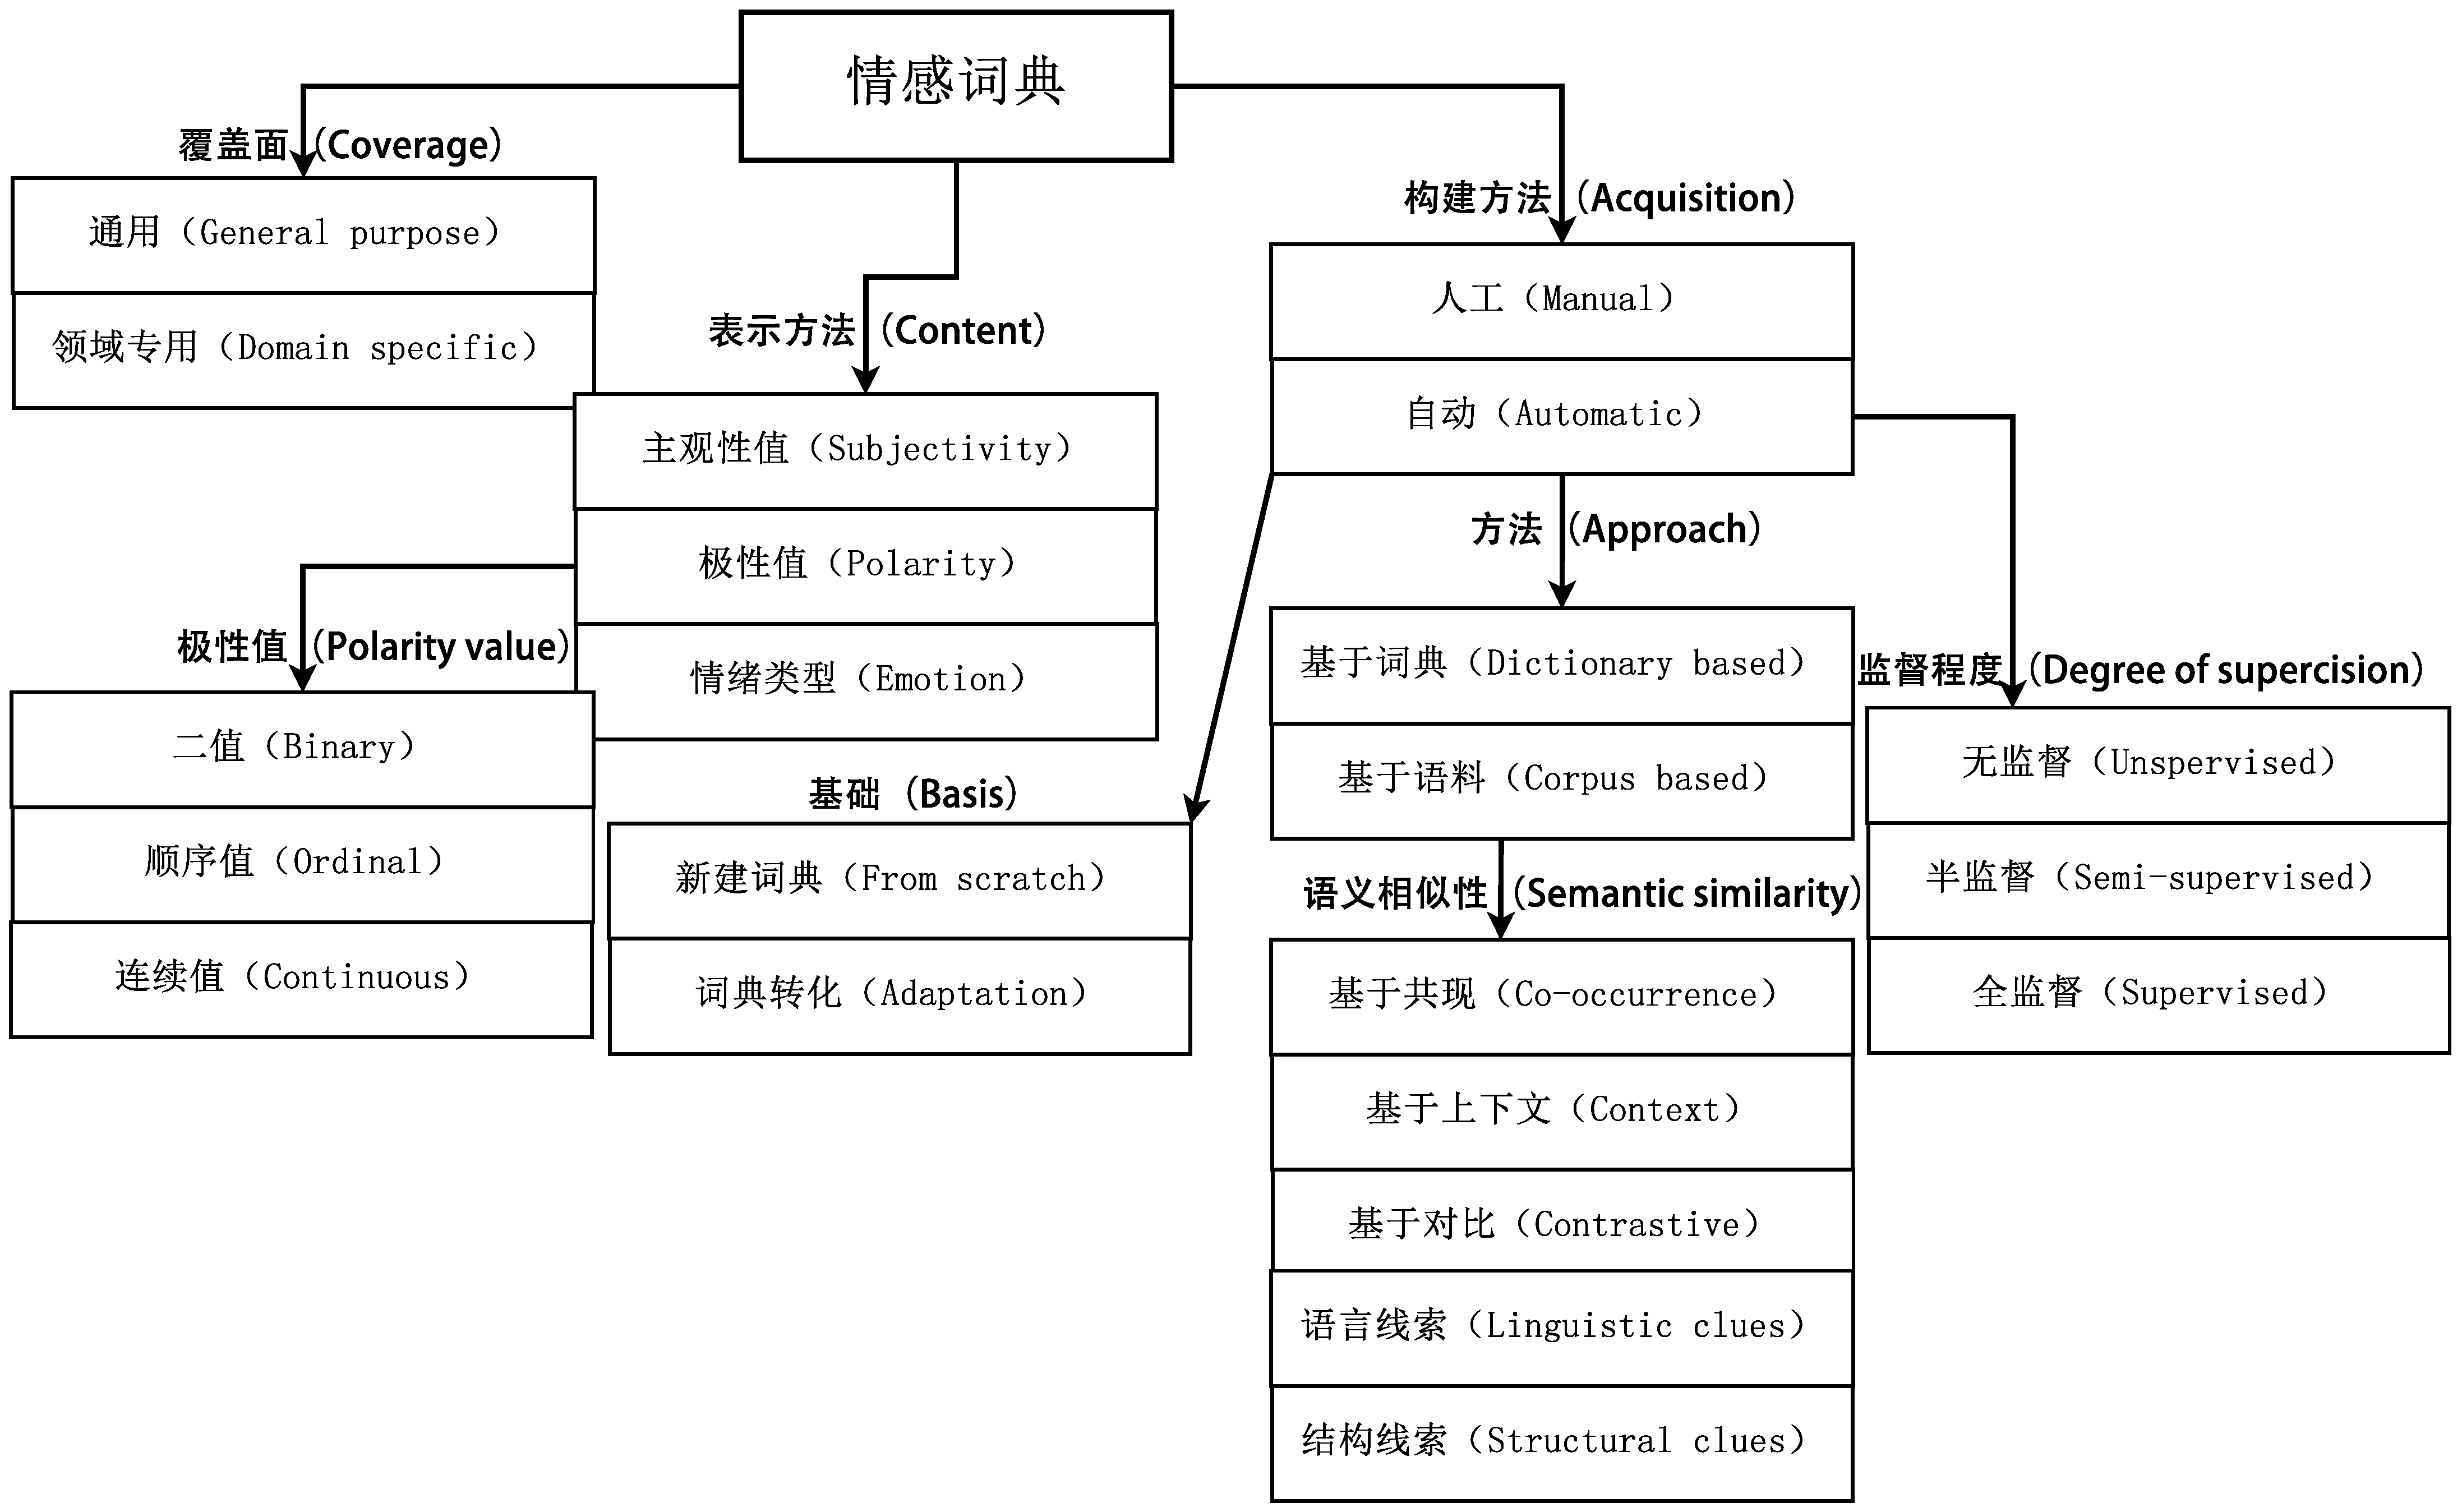
\includegraphics[height=300pt]{2-1-1.eps}
\caption{情感词典有关内容}
\label{fig2-1-1}
\end{figure}

\subsection{词典覆盖面}
就词典的覆盖面来讲,情感词典可以分为通用的词典以及领域专用的词典。构建通用情感词典的主要假设就是希望词语表达的情感独立于具体的领域和应用,这对一部分词语(比如:“赞”、“爱”、“憎恨”等),目前经常使用的情感词典基本都是通用的情感词典。但是实际上很多词语表达的情感是依赖于领域和具体的语境的,比如“轻薄”一词,一般情况表示负面情感,但是描述手机时却可以表示正面的评价。而且,一些本身不表示具体情感的词语(比如:“长”、“短”、“老”、“经典”等),用到一些特殊的语境时也会表达出一些具体情感(比如:“手机待机时间长”与“手机待机时间短”)。最近开始有一些研究开始针对具体领域和应用需求构建一些领域专用的情感词典\upcite{Choi2009,Du2010,Klenner2009}。

\subsection{词典内容}
情感词典可以就其表示情感知识内容进行细分,当然情感知识表示方法与具体的应用场景是密切相关的,我们不考虑具体的应用场景,而仅仅对词典的情感表示方法进行划分。从这个方面来看,情感词典表示情感知识的方法可以分为三种:词语表示主观性的程度(Degree of subjectivity)、表示情感的极性(Polarity)或者表示的情绪类型(Emotion\/mood,比如喜、怒、哀、乐等)。表示主观性程度的情感词典主要用于文本主观性的探测任务\upcite{CarmenBanea2008,Gyamfi2009,Maks2012,Wiebe2000,Wiebe2006},而主观文本表达观点的具体情感类型的识别,需要表示情感极性或情绪类型的情感词典。在情感分类中经常使用是表示情感极性的词典,其中的词语都标注了表达的情感极性是积极的还是消极的,这对于想要确定文本所表达观点的倾向性是非常重要的。对这类情感词典还可以根据表示的情感极性值大小进一步划分:比如使用二值情感极性(也就是积极的和消极的)的情感词典\upcite{Godbole2007,Hatzivassiloglou1997,Hu2004,Rao2009};使用顺序值(ordinal)表示极性值的情感词典,比如常使用1-5整数值区分情感极性的强度值\upcite{Yessenalina2011};还有一些使用连续数值(continuous)表示情感极性强度的情感词典\upcite{Turney2003,Sasha2008,Velikovich2010,Remus2010}。
目前有很多这样的英文情感词典,比如:OpinionFinder(OF)\upcite{Wilson2005d},Appraisal Lexicon(AL)\upcite{Taboada2004},SentiWordNet\upcite{Baccianella2010}以及Q-WordNet\upcite{Agerri2010}等。

如果为了分析更细粒度(fine-grained)的情感,需要将词语表达的情感根据情绪类型进行表示,比如Bollen等\upcite{bollen2011twitter}通过分析Twitter中大众表达出的不同情绪来预测股票指数的变化,Garcia和Schweitzer\upcite{Garcia2011}对产品评论中的情绪类型进行了细致研究,类似的工作还有Davidov等\upcite{Davidov2010}以及Strapparava和Mihalcea\upcite{Strapparava2008}在Twitter上的工作。这种类型的情感词典都是靠人工编辑形成的,比如GI(General Inquirer)\footnote{\url{http://www.wjh.harvard.edu/~inquirer/Home.html}}\upcite{Stone1966},ANEW(Affective Norms for English Words)upcite{Bradley1999},WordNet-Affect\footnote{\url{http://wndomains.fbk.eu/wnaffect.html}}upcite{Valitutti2004,Valitutti2004a},DAL (Dictionary of Affect in Language)upcite{Whissell1989}等词典。

\subsection{词典构建方法}
从情感词典的构建方法来看,可以分为人工构建和自动构建两种类型。目前公开可用的人工编辑的情感词典基本都是通用的情感词典(比如:OF词典和GI词典),人工构建情感词典主要面临的问题除了需要耗费大量的人力,还有覆盖面相对较低,以及需要对不同的领域进行适应性扩展才能达到好的观点分析效果。

而对于自动构建情感词典方法,还可以按照方法(Approach)、监督程度(Degree of supervision)和构建基础(Basis)三个维度进行区分。

\subsubsection{构建方法}
情感词典主要的构建方法分为两类:一是基于词典(dictionary-based)方法,根据已有词典的词语之间的语义关系判断词语的情感极性或计算情感极性值;二是基于语料(corpus-based)方法,根据词语在语料中的分布特点推导出情感极性并计算极性值。两类方法共同特点是都需要一个预先标注的种子词集(seed set),然后通过不断迭代计算词语与种子词集词语之间的某种语义相似性,推导词语情感极性值并扩充种子词集,直到收敛。

\paragraph{基于词典方法:}
基于词典的方法通常会使用一个词库(thesaurus)或语义知识库(比如常用的是WordNet\upcite{Miller1995}),并且常用的假设是词语间的语义关系转换词语的情感信息,最常用的语义关系是词语间的同义和反义关系\upcite{Godbole2007,Kim2006,Ahsaee2010}。例如形容词“lovely”会将积极极性通过同义关系传递给“admirable”、“adorable"”、“amiable”和“pretty”,反过来会将消极极性转换给反义词语“awful”、“unlovely”和“ugly”。但是这种转换会随着语义距离增加而弱化,比如在WordNet中从“good”到“bad”的同义关系距离长度只有3\upcite{Godbole2007},因此方法设计时需要采取适当措施将语义距离考虑在内\upcite{Godbole2007,Ide2006,Budanitsky2001,Kim2006,Ahsaee2010}。除了同义和反义关系,一些研究提出使用WordNet中的其他语义关系,比如“similarity”,“derived-from”,“pertains-to”,“also-see”或“attribute”等关系\upcite{Esuli2006,Valitutti2004a}。Takamura等\upcite{Takamura2005}以及Andreevskaia等\upcite{Andreevskaia2006}使用了并不直观的下位关系(hyponymy)构建情感词典。还有一些方法通过计算词语在词典中解释的相似性来度量词语间的语义相关性,然后根据这种语义相关性构建情感词典\upcite{Esuli2006,Baccianella2010,Takamura2007}。

\paragraph{基于语料方法:}
和基于词典方法一样,基于语料方法一个基本思想就是通过某种方法度量词语间的语义相关性,然后从标注好的种子集中推断出词语的情感信息。这些度量方法可以分为以下四种:
\begin{itemize}
\item \textbf{基于词语共现方法}:代表性的工作是Turney等\upcite{Turney2002,Turney2003},主要是假设“一个词语的语义倾向性(semantic orientation)\footnote{Turney使用语义倾向性指代词语的情感极性}往往与其相邻的词语的语义倾向性相关”,因此他们使用点互信息(pointwise mutual information)PMI统计对词语和种子词集的相关性进行度量,推导出词语的情感极性。
\item \textbf{基于上下文方法}:除了直接通过共现来度量两个词语的相关性,在统计语义学还有还有一种常用的方法就是使用词语的上下文信息。在Firth的《Contextual Theory of Meaning》一书中,提出一个基本的假设就是“a word is characterized by the company it keeps”\upcite{Firth1957},因此词语的语义信息是与上下文语境紧密相关的。因此一些基于语料的情感词典构建方法利用这一假设,提出在相似上下文出现的词语很有可能具有相似的情感信息,因此可以从情感极性已知的种子词集推导出其他词语的情感极性\upcite{Baron2003,Wiebe2000,Velikovich2010}。
\item \textbf{基于对比方法}:该类方法将前台(foreground)语料和背景(background)语料对比分析进行情感词语的抽取构建情感词典。比如Maks和Vossen\upcite{Maks2012}研究了对数似然和相对频率比提取主观词构建语情感词典,他们使用报纸新闻以及新闻评论作为主观前台语料,维基百科文本作为客观背景语料。相似的工作还有Stepinski和Mittal\upcite{Stepinski2007}。
\item \textbf{基于语言线索}:前面几种方法单纯依靠语料中统计出的信息,不考虑对文本的深层次语言学分析。其实已经有工作确认一些常用的语言模式有助于词语的情感信息的探测。Hatzivassiloglou和McKeown\upcite{Hatzivassiloglou1997}发现一个句子中连词(“and”和“but”)对与所连接的两个词语的情感极性具有一定的限制作用,出现在“and”两边的词语一般具有相同的极性,而出现在“but”两边的词语极一般性相反,他们利用这种限制从文本语料中抽取并构建情感词典。在产品评论的观点挖掘研究中一些工作扩展了这种连词语言线索,同时考虑了跨句子的连词\upcite{Ding2008,Angel,Kanayama2006,Popescu2007}。
\item \textbf{基于结构线索}:代表性的工作是Kaji和Kitsuregawa\upcite{Kaji2006,Kaji2007}的工作,他们利用HTML文档中的结构线索分别抽取情感极性为积极和消极的句子集,从大量HTML文档中抽取出大概500,000主观句子用于训练情感分类器并构建情感词典。
\end{itemize}

\subsection{词典转化}
上述的所有情感词典构建方法都是从头开始(from scratch)构建新的情感词典,最近也有一些方法研究已有情感词典进行转化,主要是增强通用情感词典的领域适应性或者从单语言情感词典扩展到多语言。通用情感词典进行领域转化方法,主要有Choi和Cardie\upcite{Choi2009}提出的基于线性规划方法,Du等\upcite{Du2010}提出的基于信息理论框架以及Qiu等\upcite{Qiu2009}使用语言模式的扩展方法等。Mihalcea等\upcite{Mihalcea2007}提出了基于词典和基于语料的方法将英文情感词典通过翻译转化为其他语言的情感词典。

\subsection{混合方法}
混合方法指的是构建情感词典时将多种词典和语料资源结合起来。例如Hoang等\upcite{Hoang2008}提出使用WordNet的语义关系产生初始情感词典,然后使用从网络语料中获取的统计信息对其进行完善,词典资源和语料资源用一个错误最小化算法(error minimization algorithm)结合起来。Lu等\upcite{Lu2011}提出将四种信息组合起来确定词语的情感极性,包括从一个通用情感词典得到的信息,从一个词库(thesaurus)得到的信息,以及从一个领域文档集中得到的语言线索和结构线索信息,这四种信息通过一个基于线性规划的优化框架结合起来确定词语的情感极性。

综上所述,目前有很多种构建情感词典方法,以针对英文资源的构建方法研究为主。中文情感词典的构建方法研究还相对较少,而且基本上是借鉴英文的构建方法,而且形成的中文情感词典表示的情感知识是简单的二值极性。本章主要研究如何从英文词典进行转化得到中文情感词典,属于词典转化方法,但是我们的实现方法是借助于双语语义知识库中的语义关系实现这种转化,而不是使用翻译的方式,而且我们形成的情感词典能够通过计算将英文情感词典的情感极性值同时转化过来,情感知识更加丰富。

%随着互联网的发展,尤其是社交网络的发展,各种社交媒体的用户发布内容中出现了海量含有用户主观情感色彩的文本数据。针对网络文本的信息处理开始由获得关键词\upcite{Yuan2013}、事件
%\upcite{张辉2013}、话题\upcite{刘健2013} 等事实信息,开始向情感观点等主观信息深入,情感分析便是近年来迅速发展的信息处理技术\upcite{Liu2012}。从数据中提炼出用户的主观信息对于商业情报、舆情分析等具有重要意义。情感分析技术就是对带有情感色彩的主观性文本进行自动推理、分析、归纳的过程,涉及自然语言处理、机器学习、认知科学以及社会心理学等方面的研究\upcite{黄萱菁2011}。


\section{词典资源简介}
\label{ch2:lex}
本节简要介绍要用到的一些词典资源。
\subsection{HowNet语义知识库}
HowNet是一个以中英文词语所代表的概念为描述对象,揭示概念与概念之间以及概念的属性与属性之间的关系的知识库\upcite{杜飞龙2000}。HowNet两个重要名词是“义原”和“概念”:概念是对词汇语义的一种描述,每一个词可以表达为几个概念\upcite{刘群2002};义原是最小语义单元,用于定义和描述概念。义原通过一个树状的层次结构组织构成上下位关系。如图~\ref{fig2-1}所示,HowNet采用KDML(Knowledge Dictionary Mark-up Language)语言描述概念,其中W\_X表示词语,G\_X表示词语词性,E\_X表示词语例子,X为C时表示中文,X为E时表示英文。DEF是对于该概念的定义项,称之为一个语义表达式,其中中英文标注的是义原,“\#\*”等标示符号来对概念属性之间关系进行描述,DEF中还可以包含概念,概念之间相互交织构成一个网。HowNet一共有2234个义原,收录了近15万条概念记录,涵盖了绝大部分中文常用词语,本章将基于HowNet的词语进行情感词典的构建。

\begin{figure}[htp]
\centering
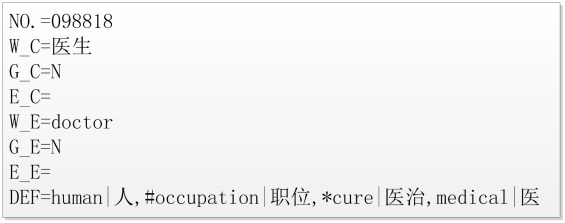
\includegraphics[height=120pt]{2-1.png}
\caption{HowNet中概念的定义方式}
\label{fig2-1}
\end{figure}

\subsection{WordNet语义词典}
WordNet是由Princeton大学的心理学家,语言学家和计算机工程师联合设计的一种基于认知语言学的英文词典\upcite{Fellbaum1998}。WordNet是根据词义而不是词形来组织词汇信息。WordNet使用同义词集合(Synset)代表概念,词汇关系在词语之间体现,语义关系在概念之间体现。WordNet将英语的名词、动词、形容词和副词组织为Synsets,每一个Synset表示一个基本的词汇概念,并在这些概念之间建立了包括同义关系(synonymy)、反义关系(antonymy)等多种语义关系。其中,WordNet最重要的关系就是词的同义反义关系。

\subsection{SentiWordNet情感词典}
SentimentWordNet是Baccianella\upcite{Baccianella2010}等在语义词典WordNet基础上使用随机游走的图算法得到的情感词典。词典的每条记录都是一个WordNet的Synset,并且每个Synset都计算出了褒义、贬义情感强度值,本文就是利用SentimentWordNet的情感强度值以及HowNet概念的语义关系进行计算得到中文词语的情感极性值。SentimentWordNet共有117,000多 Synsets,192,493单词。

\section{基于语义关系的情感词典构建方法}
\label{ch2:construct}
将英文情感词典的研究成果转化为文资源,可以利用语言之间的语义对应关系减少词典的歧义,使情感词典更加可靠,还可以直接将英文中对情感强度的计算直接转化为中文词语的情感强度计算,减少了计算开支。本研究正是基于这种动机展开的。HowNet对义原和概念进行了英汉双语标注,可以作为转化的“桥梁”。但是英文词语和中文词语都存在一词多义现象,不同语义所表达的情感倾向也不同,因此得到的情感极性值也会存在歧义。HowNet中概念的DEF是由义原按语义关系进行描述的,可以利用这种语义关系对词语的情感极性值进行“消歧”。总体来说,解决方案如图~\ref{frame}框架所示。

\begin{landscape}
\begin{figure*}
\centering
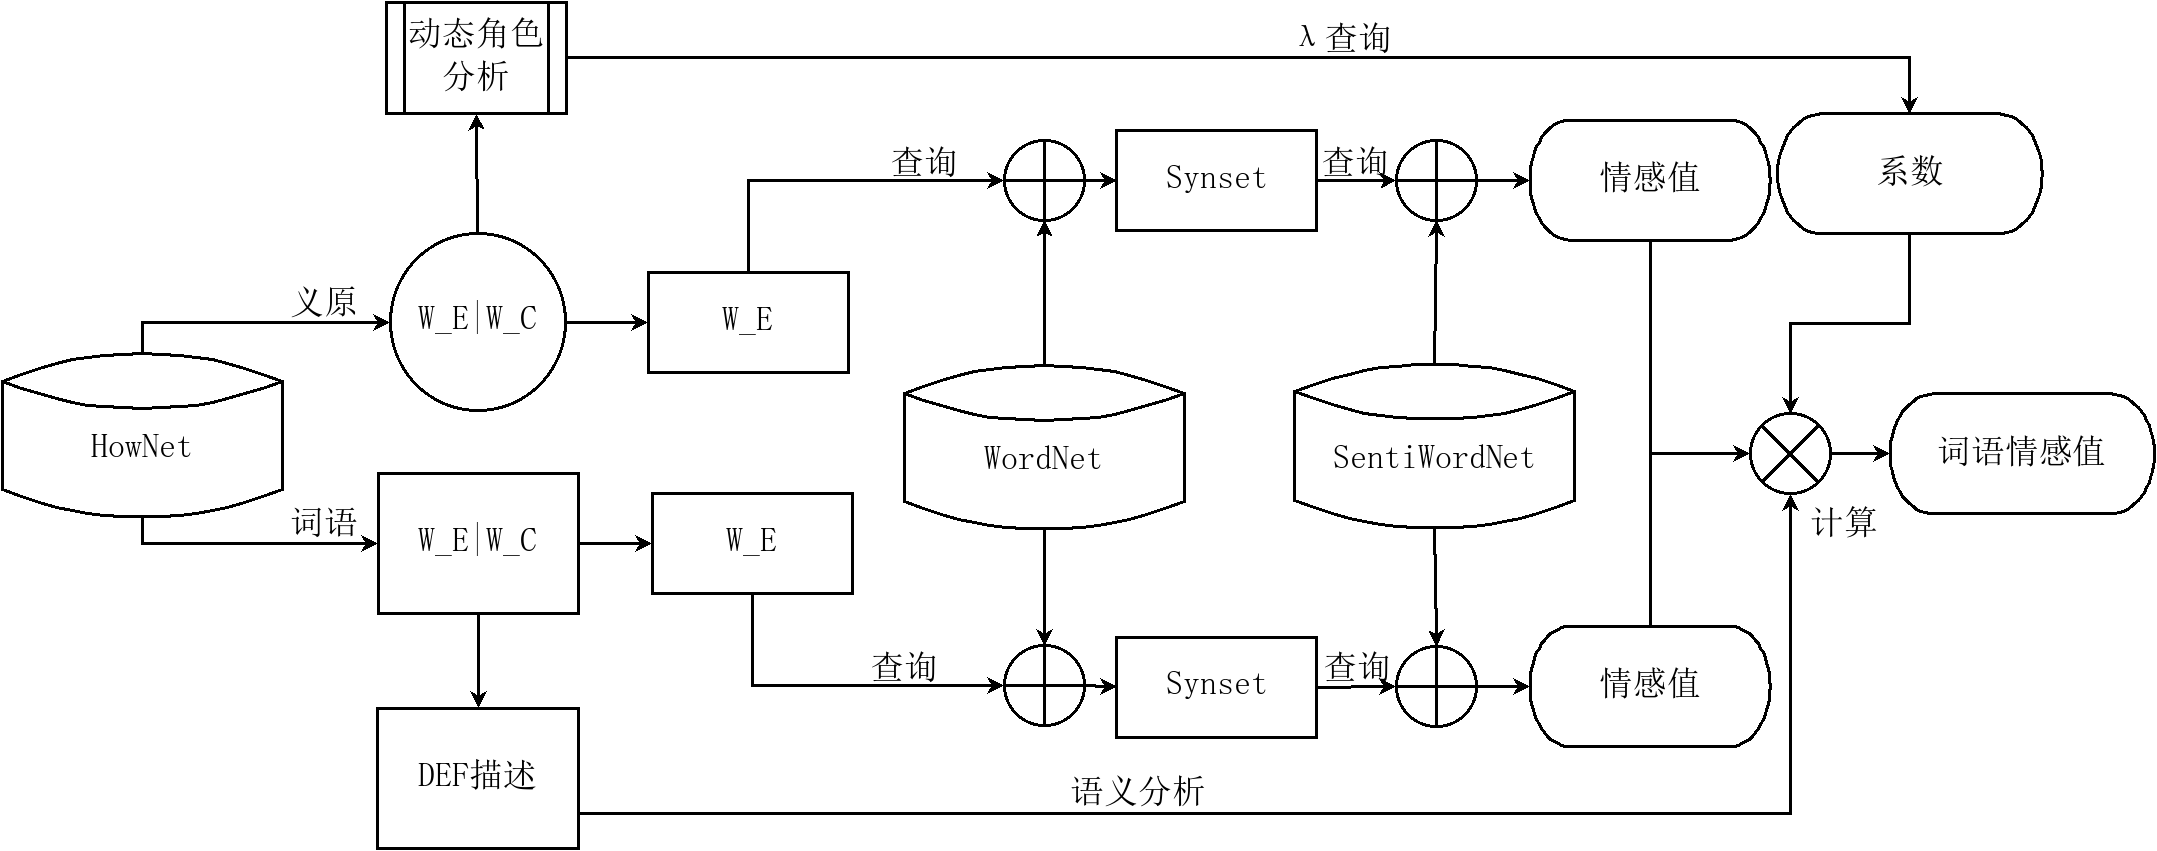
\includegraphics[height=280pt]{2-2.png}
\caption{基于语义关系的情感词典解决方案}
\label{frame}
\end{figure*}
\end{landscape}
构建中文情感词典框架可以分为义原和词语抽取及语义分析、义原和词语情感极性值查询与计算以及词语的情感极性值计算三个过程。

\subsection{词语抽取和义原抽取及语义分析}
词语抽取主要是从HowNet词典中抽取词语(W\_C)和属性定义(DEF)并对DEF进行分析。DEF是由义原和语义关系描述等构成的,在进行词语倾向计算时,需要根据义原进行词语的语义分析和倾向计算。情感词语抽取处理流程如图~\ref{atom}所示。

\begin{figure}[htp]
\centering
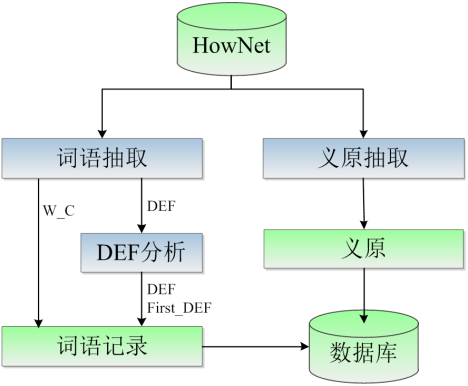
\includegraphics[height=170pt]{2-3.png}
\caption{词语和义原抽取处理流程}
\label{atom}
\end{figure}

在抽取得到的词语记录中,主要关注的内容有词语编号(No\.)、中文词语(W\_C)、中文词性(G\_C)、英文词语(W\_E)、英文词性(G\_E)、属性(DEF)、第一属性(First\_DEF)等。其中第一属性是指位于属性DEF第一位置的义原,通过第一属性可以分析出该词语所属的特征类。

由于HowNet中的词语是由义原和语义关系描述等构成的。在进行词语倾向计算时,需要根据义原进行词语的语义分析和倾向计算。在抽取得到的义原的记录中,主要关注的内容有词语编号(No\.)、特征类别(Category)、中文词语(W\_C)、英文词语(W\_E)、属性(DEF)、层次(Layer)、父亲节点编号(Father)等。根据记录中的层次(Layer)和父亲节点编号(Father)可以得到义原之间的语义关系,如编号为33的义原“依靠”位于“事件类(Event)”的第五层,其父亲节点编号为32,通过查询编号为32的义原,得到其父亲节点义原为“有关(relate)”,表示DEF中包含,因此抽取的记录中包含了义原及其在词语中的语义关系。

\subsection{情感极性值的查询与计算}
HowNet词语是中英双语,因此有的可以直接将抽取到的英文词语(W\_E)、英文词性(G\_E)直接送入英文情感词典查询其情感极性值。但是大部分词语英文部分不是一个单词,因此无法直接得到情感极性值,而且由于词语的多义性,也无法获得唯一的情感极性值,因此需要进行“消歧”;HowNet中词语是由其属性DEF定义的,DEF是由多个义原按照一定的语义关系组合而成的,词语的倾向性可以看作是由义原的倾向性按照一定的规律组合而成的。因此词语的倾向性值可以通过义原的倾向性值根据语义关系计算获得,一方面可以获得直接查询无法获得情感极性值的词语,另外一方面也可以利用DEF情感极性值进行修正并消歧。

\subsubsection{词语倾向性值查询与计算}
\label{sense}
WordNet是以词义(sense)来记录的, sense以同一词义的词集Synset表示。通过查询可以得到词语W\_E所有的sense,将每个sense映射到SentiWordNet就可以得到对应的情感极性值。

\subsubsection{义原倾向性值查询与计算}
基于WordNet和SentiWordNet的义原倾向计算过程如图~\ref{atomsen}所示。
在HowNet中获取义原后将义原对应英文词语(如“good”)映射到WordNet中进行查询,得到该词语所有的Sense(如“good”的Sense共有27个);将这些Sense映射到SentiWordNet中查询得到对应Sense情感极性值;将情感极性值加权根据公式~\ref{eq1}计算得到义原的情感倾向值(如“good”的倾向值为PosScore=0.597,NegScore=0.004)。
\begin{equation}
\label{eq1}
\varphi(s,p)=\dfrac{\sum_{i=1} \varphi_i (s,p)}{\sum_{p\in P}\sum_{i=1}^m \varphi_i(s,p)}
\end{equation}

\begin{figure}[htp]
\centering
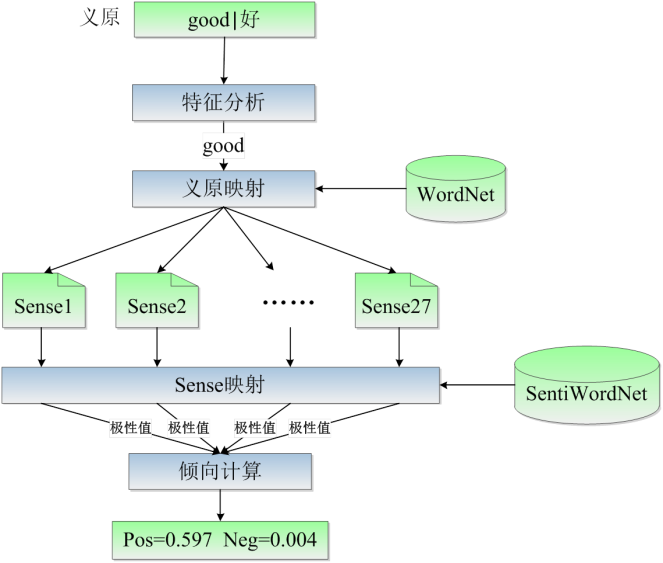
\includegraphics[height=250pt]{2-4.png}
\caption{义原情感极性值计算过程}
\label{atomsen}
\end{figure}

公式中$ P$表示极性类型(积极、消极、中性,“P、N、O”),$m$为与义原相对应的Sense的总数,$s$表示义原,$\varphi(s,p)$表示义原的极性值,$\varphi_i (s,p)$表示义原在编号为的Sense中的类型极性值。

事件类义原有很多在DEF描述中可以引起情感极性值的变化,比如“DoNot|不做,lose|失去”等会引起情感极性值符号反转,因此我们标注了819个事件类义原的在情感极性值计算中的语义角色,并用系数$\lambda$来表示。

\subsection{词语情感极性值计算}
通过~\ref{sense}部分查询可以获得部分词语的情感倾向值,有些词语由于是多义的,情感极性值可能有几个,因此需要根据词语DEF描述中义原情感极性值进行计算修正和消歧。对HowNet中词语属性描述DEF语义关系的不同提出如下定义:

\textbf{定义1 情感倾向值取反:}词语$s$的$p$极性值$\varphi(s,p)$取反运算是,将$s$的积极倾向值和消极倾向值互换,过程如公式~\ref{2-2}:
\begin{equation}
\label{2-2}
\overline{\varphi(s,p)}=\varphi(s,p),\quad (p,q) \in P\&\& p \neq q
\end{equation}

\textbf{定义2 因子乘法运算:} $\lambda$因子与词语$s$的$p$极性值的乘法运算定义为$\lambda$乘法运算,过程如公式~\ref{2-3}:
\begin{equation}
\label{2-3}
\lambda \times \varphi(s,p) =\begin{cases}
& \lambda \varphi(s,p), \quad  \lambda >0\\
& 0, \quad\quad  \lambda=0\\
&|\lambda|\varphi(s,p), \quad  \lambda <0
\end{cases}
\end{equation}
$\lambda$取值的确定需要根据义原的类别特征、词语DEF的组成特征和义原间的语义关系进行确定,这些都已经在抽取部分和义原情感极性值计算部分记录下来。如词语“好”的DEF中每个义原的$\lambda$可以均取值为1。词语“扭亏为盈”的DEF为“DEF=alter|改变,StateIni=InDebt|亏损,StateFin=earn|赚”,义原“InDebte|亏损”为初始状态,“earn|赚”为最终状态,经过分析后,义原“InDebte|亏损”的$\lambda$取值为0,义原“earn|赚”的$\lambda$取值为1。词语倾向计算总结为公式~\ref{2-4}。其中$\varphi(s,p)$表示词语$s$的$p$极性值,$t_i$表示词语DEF中第$i$个义原,$n$为词语DEF中义原总数。
\begin{equation}
\label{2-4}
\varphi(s,p)=\dfrac{\sum_{i=1}^n\lambda_i\times\varphi(t_i,p)}{\sum_{p\in P}\sum_{i=1}^n\lambda_i\times\varphi(t_i,p)}
\end{equation}
其中:$\sum_{p \in P}\varphi(s,p)=1$。

对于已经通过查询得到情感极性值的词语,可以在多个英文词义sense对应的情感极性值$\varphi(s,p)$取最接近DEF分析计算得到的情感极性值$\varphi_min(s,p)$的,然后加和平均,计算公式为:
\begin{equation}
\Psi(s,p)=\dfrac{\varphi_{min}(s,p)+\varphi(s,p)}{2}
\end{equation}
其中:$\varphi_{min}(s,p)=\min \{|\varphi_s(s,p)-\varphi(s,p)|\}$。

\section{实验及结果}
情感词典的实验评测有两种方法,一是与人工编辑的或者其他可靠性较高的词典进行对比评测,二是将词典应用到情感分析的其他任务上观察性能的提升,本文使用第一种方法。在实验评测时,基准词语由HowNet中随机选取了2000个词语进行人工判断,人工判断只给出褒贬两种极性。本章生成词典SentiLex与HowNet情感词典,NTUSD情感词典以及大连理工大学的情感词汇本体词库DLLEX进行对比评价。

\subsection{评价指标}
评价指标采用准确率、召回率以及F值作为评测标准。设$a_1$表示褒义判断正确词数;$a_2$表示贬义判断正确词数;$b_1$表示判断为褒义的词数;$b_2$表示判断为贬义词数;$c_1$表示基准词典褒义词数;$c_12$表示基准词典贬义词数。准确率计算公式为:$$P=\dfrac{a_1+a_2}{b_1+b_2}\times 100\%$$
召回率计算公式为:$$R=\dfrac{a_1+a_2}{c_1+c_2}\times 100\%$$
F值计算公式为:$$F=\dfrac{2 \times P\times R}{P+R} \times100\%$$

\subsection{性能评测结果}
\subsubsection{阈值T的设定}
由于基准词是褒贬二值标注的,因此需要将生成的情感词典连续情感极性值转换为离散褒贬值。将褒义和贬义情感极性值相减得到词语的倾向值来判断词语的极性,为了提高判断的准确性,设定阈值T,高于T为褒义,低于-T为贬义。图\ref{fig2-5}为T的不同取值对词典性能指标的影响。在T=0时,虽然召回率最高达到88.58\%,但准确率最低仅有54.40\%,F值仅为67.40\%。挡T=0.05时,准确率提高到77.75\%,有较大提高,召回率仅下降到87.61\%,下降幅度较小,F值提高到82.39\%。当T提高到0.05时性能指标达到最好,因此可以设定T为0.05。

\begin{figure}[htp]
\centering
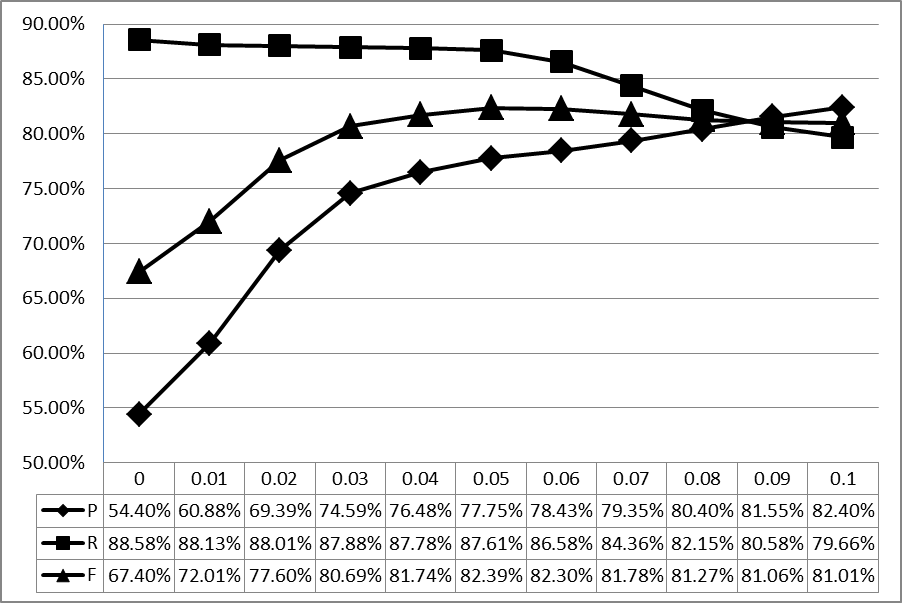
\includegraphics[height=250pt]{2-5.png}
\caption{不同T值时的性能指标}
\label{fig2-5}
\end{figure}

\subsubsection{与其他词典性能对比}
在T=0.05时,SentiLex与其他词典性能比较如表~\ref{tab2-1}所示,SentiLex准确率为77.75\%,接近最高的DLLEX词典78.40\%,而召回率为87.61\%,F值为82.39\%,均为四个词典中最高。
\begin{table}[htp]
\centering
\caption{T=0.05时的性能对比}
\label{tab2-1}
 \begin{tabular}{|l|l|l|l|}
 \hline
 &准确率(P)& 召回率(R)&F值\\
 \hline
 HowNet &74.55\%&82.35\%&78.26\%\\
NTUSD&64.23\%&80.27\%&71.36\%\\
DLLEX&\textbf{78.40\%}&85.58\%&81.83\%\\
SentiLex&77.75\%&\textbf{87.61\%}&\textbf{82.39\%}\\
 \hline
\end{tabular}
\end{table}

\section{小结}
本章对中文情感词典构建相关研究进行了分析,以英文情感词典为基础,设计了基于语义关系的情感词典自动构建方法。方法以HowNet、WordNet语义词典和SentiWordNet情感词典为基础,借鉴英文情感词典进行中文情感词典的构建,并且与现有的常用情感词典进行了实验对比。实验结果表明,本文设计的方法取得了较好的评测性能。